\documentclass[a0paper,landscape,final]{baposter}

\usepackage{times}
\usepackage{calc}
\usepackage{graphicx}
\usepackage{amsmath}
\usepackage{amssymb}
\usepackage{relsize}
\usepackage{multirow}
\usepackage{bm}
\usepackage{tkz-berge}
\usepackage[upright]{fourier}
\usepackage{bm}
\usepackage{caption}

\usepackage{graphicx}
\usepackage{multicol}

\usepackage{pgfbaselayers}
\pgfdeclarelayer{background}
\pgfdeclarelayer{foreground}
\pgfsetlayers{background,main,foreground}

\usepackage{helvet}
%\usepackage{bookman}
\usepackage{palatino}

%\newcommand{\captionfont}{\footnotesize}

\selectcolormodel{cmyk}

\graphicspath{{images/}}

%%%%%%%%%%%%%%%%%%%%%%%%%%%%%%%%%%%%%%%%%%%%%%%%%%%%%%%%%%%%%%%%%%%%%%%%%%%%%%%%
%%%% Some math symbols used in the text
%%%%%%%%%%%%%%%%%%%%%%%%%%%%%%%%%%%%%%%%%%%%%%%%%%%%%%%%%%%%%%%%%%%%%%%%%%%%%%%%
% Format 
\newcommand{\Matrix}[1]{\begin{bmatrix} #1 \end{bmatrix}}
\newcommand{\Vector}[1]{\Matrix{#1}}
\newcommand*{\SET}[1]  {\ensuremath{\mathcal{#1}}}
\newcommand*{\MAT}[1]  {\ensuremath{\mathbf{#1}}}
\newcommand*{\VEC}[1]  {\ensuremath{\bm{#1}}}
\newcommand*{\CONST}[1]{\ensuremath{\mathit{#1}}}
\newcommand*{\norm}[1]{\mathopen\| #1 \mathclose\|}% use instead of $\|x\|$
\newcommand*{\abs}[1]{\mathopen| #1 \mathclose|}% use instead of $\|x\|$
\newcommand*{\absLR}[1]{\left| #1 \right|}% use instead of $\|x\|$

\def\norm#1{\mathopen\| #1 \mathclose\|}% use instead of $\|x\|$
\newcommand{\normLR}[1]{\left\| #1 \right\|}% use instead of $\|x\|$

\makeatletter
\newcommand*{\Tiny}{\@setfontsize\Tiny{12pt}{13pt}}
\makeatother

%%%%%%%%%%%%%%%%%%%%%%%%%%%%%%%%%%%%%%%%%%%%%%%%%%%%%%%%%%%%%%%%%%%%%%%%%%%%%%%%
% Multicol Settings
%%%%%%%%%%%%%%%%%%%%%%%%%%%%%%%%%%%%%%%%%%%%%%%%%%%%%%%%%%%%%%%%%%%%%%%%%%%%%%%%
\setlength{\columnsep}{0.7em}
\setlength{\columnseprule}{0mm}


%%%%%%%%%%%%%%%%%%%%%%%%%%%%%%%%%%%%%%%%%%%%%%%%%%%%%%%%%%%%%%%%%%%%%%%%%%%%%%%%
% Save space in lists. Use this after the opening of the list
%%%%%%%%%%%%%%%%%%%%%%%%%%%%%%%%%%%%%%%%%%%%%%%%%%%%%%%%%%%%%%%%%%%%%%%%%%%%%%%%
\newcommand{\compresslist}{%
\setlength{\itemsep}{1pt}%
\setlength{\parskip}{0pt}%
\setlength{\parsep}{0pt}%
}


%%%%%%%%%%%%%%%%%%%%%%%%%%%%%%%%%%%%%%%%%%%%%%%%%%%%%%%%%%%%%%%%%%%%%%%%%%%%%%
%%% Begin of Document
%%%%%%%%%%%%%%%%%%%%%%%%%%%%%%%%%%%%%%%%%%%%%%%%%%%%%%%%%%%%%%%%%%%%%%%%%%%%%%

\begin{document}

%%%%%%%%%%%%%%%%%%%%%%%%%%%%%%%%%%%%%%%%%%%%%%%%%%%%%%%%%%%%%%%%%%%%%%%%%%%%%%
%%% Here starts the poster
%%%---------------------------------------------------------------------------
%%% Format it to your taste with the options
%%%%%%%%%%%%%%%%%%%%%%%%%%%%%%%%%%%%%%%%%%%%%%%%%%%%%%%%%%%%%%%%%%%%%%%%%%%%%%
\typeout{Poster Starts}
\background{
  \begin{tikzpicture}[remember picture,overlay]%
    \draw (current page.north west)+(-2em,-0em) node[anchor=north west] {\hspace{-2em}
\includegraphics[height=1.1\textheight]{silhouettes_background}};
  \end{tikzpicture}%
}
\definecolor{silver}{cmyk}{0,0,0,0.3}
\definecolor{yellow}{cmyk}{0,0,0.9,0.0}
\definecolor{reddishyellow}{cmyk}{0,0.22,1.0,0.0}
\definecolor{black}{cmyk}{0,0,0.0,1.0}
\definecolor{darkYellow}{cmyk}{0,0,1.0,0.5}
\definecolor{darkSilver}{cmyk}{0,0,0,0.1}

\definecolor{lightyellow}{cmyk}{0,0,0.3,0.0}
\definecolor{lighteryellow}{cmyk}{0,0,0.1,0.0}
\definecolor{lighteryellow}{cmyk}{0,0,0.1,0.0}
\definecolor{lightestyellow}{cmyk}{0,0,0.05,0.0}
\begin{poster}{
  % Show grid to help with alignment
  grid=false,
  % Column spacing
  colspacing=1em,
  % Color style
  bgColorOne=lighteryellow,
  bgColorTwo=lightestyellow,
  borderColor=reddishyellow,
  headerColorOne=lightyellow,
  headerColorTwo=silver,
  headerFontColor=black,
  boxColorOne=lightestyellow,
  boxColorTwo=lightestyellow,
  % Format of textbox
  textborder=roundedleft,
  % Format of text header
  eyecatcher=false,
  headerborder=open,
  headerheight=0.08\textheight,
  headershape=roundedright,
  headershade=plain,
  headerfont=\Tiny, %\textsf, %Sans Serif
  boxshade=plain,
%  background=shade-tb,
  background=plain,
  linewidth=1pt
  }
  % Eye Catcher
  {} % No eye catcher for this poster. If an eye catcher is present, the title is centered between eye-catcher and logo.
  % Title
  {\sf %Sans Serif
  %\bf% Serif
  \vspace{0.5em}
  Unsupervised Feature Learning for Object Classification
  \vspace{0.2em}
  }
  % Authors
  {\sf %Sans Serif
  % Serif
  Laxman Dhulipala, Harry Gifford, Wangzi He\hspace{3em}
  \{ldhulipa, hgifford, wangzih\}@andrew.cmu.edu\hspace{3em}
  }
  % University logo
  {{\begin{minipage}{25em}
    \hfill
%    
\includegraphics[height=2em]{msrlogo}
%    
\includegraphics[height=5.5em]{logo}
%     
\includegraphics[width=20em]{cmu_seal}
     \vspace{0.2em}
     
\includegraphics[height=5.5em]{seal}
  \end{minipage}}
  }

  \tikzstyle{light shaded}=[top color=baposterBGtwo!30!white,bottom color=baposterBGone!30!white,shading=axis,shading angle=30]

  % Width of left inset image
     \newlength{\leftimgwidth}
     \setlength{\leftimgwidth}{0.78em+8.0em}

%%%%%%%%%%%%%%%%%%%%%%%%%%%%%%%%%%%%%%%%%%%%%%%%%%%%%%%%%%%%%%%%%%%%%%%%%%%%%%
%%% Now define the boxes that make up the poster
%%%---------------------------------------------------------------------------
%%% Each box has a name and can be placed absolutely or relatively.
%%% The only inconvenience is that you can only specify a relative position 
%%% towards an already declared box. So if you have a box attached to the 
%%% bottom, one to the top and a third one which should be in between, you 
%%% have to specify the top and bottom boxes before you specify the middle 
%%% box.
%%%%%%%%%%%%%%%%%%%%%%%%%%%%%%%%%%%%%%%%%%%%%%%%%%%%%%%%%%%%%%%%%%%%%%%%%%%%%%
    %
    % A coloured circle useful as a bullet with an adjustably strong filling
    \newcommand{\colouredcircle}[1]{%
      \tikz{\useasboundingbox (-0.2em,-0.32em) rectangle(0.2em,0.32em); \draw[draw=black,fill=baposterBGone!80!black!#1!white,line width=0.03em] (0,0) circle(0.18em);}}

%%%%%%%%%%%%%%%%%%%%%%%%%%%%%%%%%%%%%%%%%%%%%%%%%%%%%%%%%%%%%%%%%%%%%%%%%%%%%%
  \headerbox{Contribution}{name=contribution,column=0,row=0}{
%%%%%%%%%%%%%%%%%%%%%%%%%%%%%%%%%%%%%%%%%%%%%%%%%%%%%%%%%%%%%%%%%%%%%%%%%%%%%%
   {}
   
   We implement an unsupervised method for learning features from images,
   which are then used for image classification. Our method is robust, and
   we experimentally show its performance on the CIFAR-10 dataset, a standard
   dataset in the machine learning community.
 }
 
 %%%%%%%%%%%%%%%%%%%%%%%%%%%%%%%%%%%%%%%%%%%%%%%%%%%%%%%%%%%%%%%%%%%%%%%%%%%%%%
  \headerbox{Problem}{name=problem,column=0,below=contribution}{
%%%%%%%%%%%%%%%%%%%%%%%%%%%%%%%%%%%%%%%%%%%%%%%%%%%%%%%%%%%%%%%%%%%%%%%%%%%%%%
    Finding a robust and compact set of features is a fundamental problem
    in machine learning, with applications to a number of applications, including
    classification and similarity-detection. Finding a compact basis for represnting
    images is therefore one of the first tasks faced by both academics and industry scientists
    working on image classification. 
%   We want to learn feature representation for data with arbitrary form when 
%   the number of unlabeled data is much more than the number of labeled data.
 }
 
 %%%%%%%%%%%%%%%%%%%%%%%%%%%%%%%%%%%%%%%%%%%%%%%%%%%%%%%%%%%%%%%%%%%%%%%%%%%%%%
  \headerbox{Motivation}{name=motivation,column=0,below=problem}{
%%%%%%%%%%%%%%%%%%%%%%%%%%%%%%%%%%%%%%%%%%%%%%%%%%%%%%%%%%%%%%%%%%%%%%%%%%%%%%
   Representing an $n \times n$ image using all $n^{2}$ pixels is almost
   always highly-wasteful of computational resources. This is due to two neighboring
   pixels being highly correlated, as they are likely to have very similar RGBA values.
   Learning more general features allows us to represent data in a much more 
   efficient manner, and reduces both the memory and space utilization of machine
   learning algorithms. 
 }

%%%%%%%%%%%%%%%%%%%%%%%%%%%%%%%%%%%%%%%%%%%%%%%%%%%%%%%%%%%%%%%%%%%%%%%%%%%%%%
  \headerbox{Methodology}{name=method,column=0,below=motivation}{
%%%%%%%%%%%%%%%%%%%%%%%%%%%%%%%%%%%%%%%%%%%%%%%%%%%%%%%%%%%%%%%%%%%%%%%%%%%%%%
    Our approach involves a  steps to learn a feature representation. We
    are going to explain each step in the following sections.  
  }

%%%%%%%%%%%%%%%%%%%%%%%%%%%%%%%%%%%%%%%%%%%%%%%%%%%%%%%%%%%%%%%%%%%%%%%%%%%%%%
  \headerbox{Preprocessing}{name=preprocess,column=0,below=method, above=bottom}{
%%%%%%%%%%%%%%%%%%%%%%%%%%%%%%%%%%%%%%%%%%%%%%%%%%%%%%%%%%%%%%%%%%%%%%%%%%%%%%
    1. We extract random patches (8 $\times$ 8) from unlabeled training images.\\
    2. We apply PCA on those patches to reduce feature dimensions since each pixel 
       is a feature in the original patch. (Optional step) \\
    3. Normalize data so that mean is zero and variance is one. \\ 
    4. We whiten data to eliminate correlations between neighboring pixels. (Neighboring
       pixels tend to have similar colors.)  
  }

%%%%%%%%%%%%%%%%%%%%%%%%%%%%%%%%%%%%%%%%%%%%%%%%%%%%%%%%%%%%%%%%%%%%%%%%%%%%%%
  \headerbox{Clustering}{name=clustering,column=1,row=0}{
%%%%%%%%%%%%%%%%%%%%%%%%%%%%%%%%%%%%%%%%%%%%%%%%%%%%%%%%%%%%%%%%%%%%%%%%%%%%%%
    We run K-Means on the preprocessed patches, using a predetermined parameter $k$. 
    We want to select $k$ to be as large as possible without having many
    singular clusters where a singular cluster is a cluster with no elements or very 
    few elements in it. Clusters are computed using the $l_2$ norm, although other
    metrics such as cosine-distance can easily be used.~\cite{coates}\\ 
  }

%%%%%%%%%%%%%%%%%%%%%%%%%%%%%%%%%%%%%%%%%%%%%%%%%%%%%%%%%%%%%%%%%%%%%%%%%%%%%%
  \headerbox{Centroids as Features}{name=imageDisp,column=1,row=0, below=clustering, above=bottom}{
%%%%%%%%%%%%%%%%%%%%%%%%%%%%%%%%%%%%%%%%%%%%%%%%%%%%%%%%%%%%%%%%%%%%%%%%%%%%%%
  Learned features show noticable similarities to Gabor wavelets, and
  patterns exhibited by neurons in the $V1$ cortex of the brain. 

%\begin{center}
%  \includegraphics{filename}
%    \captionof{figure}{text}
%      \label{fig:name}
%      \end{center}
%
  \begin{center}
  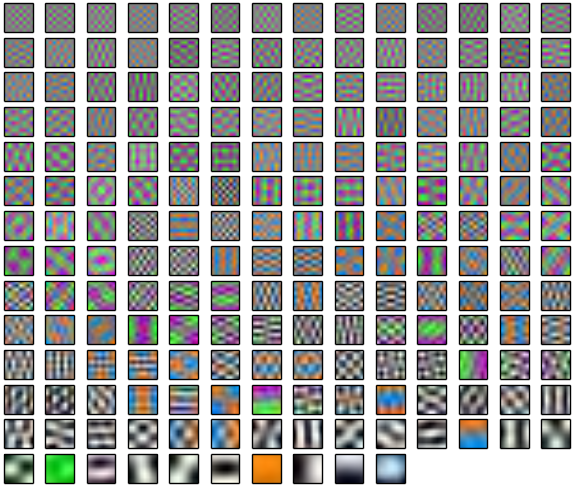
\includegraphics[width=0.6\colwidth]{figs/eigs192.png}
  \captionof{figure}{All 192 eigenvectors from a selection of $8 \times 8$ patches.}
  \end{center}

  \begin{center}
  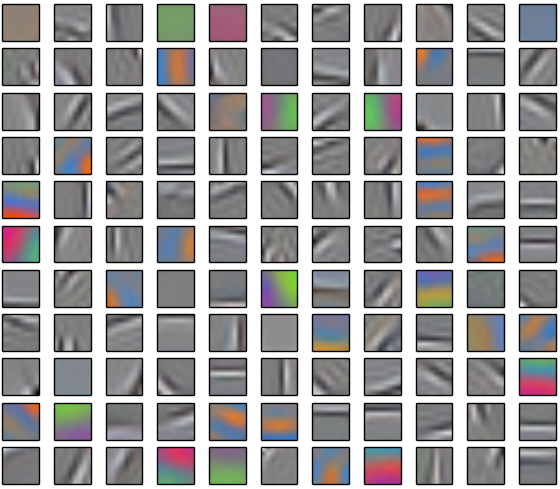
\includegraphics[width=0.5\colwidth]{figs/patches100.png}
  \captionof{figure}{100 centroids learnt from applying $K$-means to $8 \times 8$ patches.}
  \end{center}
  }
  
   
%%%%%%%%%%%%%%%%%%%%%%%%%%%%%%%%%%%%%%%%%%%%%%%%%%%%%%%%%%%%%%%%%%%%%%%%%%%%%%
  \headerbox{Pooling}{name=pooling,column=2,row=0}{
%%%%%%%%%%%%%%%%%%%%%%%%%%%%%%%%%%%%%%%%%%%%%%%%%%%%%%%%%%%%%%%%%%%%%%%%%%%%%%
  1. For each labeled image, we extract all possible patches for it.\\
  2. Each patch extracted will correspond to a K-dimension vector. Let the 
  	 vector corresponding to the i$^{\text{th}}$ patch be $v_i$. Element $v_{ij}$ equals 
  	 max(0, $\mu_i$ - $x_{ij}$) where $\mu_i$ is the average distance from the
  	 patch to each centroid and $x_{ij}$ is the distance from patch i to 
  	 centroid j.\\
  3. We divide those patches into n groups and sum over each single column of the data 
     in each group. We will obtain n $\times$ K values and those will be the new features.
  Finally, images are classified as follows:

  }
  
%%%%%%%%%%%%%%%%%%%%%%%%%%%%%%%%%%%%%%%%%%%%%%%%%%%%%%%%%%%%%%%%%%%%%%%%%%%%%%
  \headerbox{Classification}{name=classification,column=3, row=0}{
%%%%%%%%%%%%%%%%%%%%%%%%%%%%%%%%%%%%%%%%%%%%%%%%%%%%%%%%%%%%%%%%%%%%%%%%%%%%%%
  1. Divide labeled data into training and test sets. \\
  2. Pass these new features into SVM or other classifiers. 
  } 
  
%%%%%%%%%%%%%%%%%%%%%%%%%%%%%%%%%%%%%%%%%%%%%%%%%%%%%%%%%%%%%%%%%%%%%%%%%%%%%%
  \headerbox{Results}{name=results,column=2,span=2,below=classification, below=pooling}{
%%%%%%%%%%%%%%%%%%%%%%%%%%%%%%%%%%%%%%%%%%%%%%%%%%%%%%%%%%%%%%%%%%%%%%%%%%%%%%
      \begin{multicols}{2}
        The method was evaluated on the GavabDB expression dataset which
        contains 427 Scans, with 3 neutral scans and 4 expression scans per ID.
        To test the impact of expression invariance on neutral data we used the
        UND Dataset from the Face Recognition Great Vendor Test, which contains
        953 neutral scans with one to eight scans per subject.
      \end{multicols}\vspace{-1em}
%      \mbox{\hspace{0.3\linewidth}\rule{0.4\linewidth}{1pt}\hspace{0.3\linewidth}}\\
%      \begin{tabular}{cc}
%        \hspace{0.5em}\scalebox{0.74}{\input{shrec_MNCG}} &
%        \hspace{0.5em}\scalebox{0.74}{\input{und_MNCG}}
%      \end{tabular}\\
        {Expression neutralization improves results on the expression dataset
        without decreasing the accuracy on the neutral testset. Plotted is the
        ratio of correct answers to  the number of possible correct answers.
        %Note the different scales for the two graphs.
        %Our approach has a high accuracy on the neutral (UND) dataset.
        }
%      \end{multicols}\vspace{-1em}
      \\\mbox{\hspace{0.3\linewidth}\rule{0.4\linewidth}{1pt}\hspace{0.3\linewidth}}\\
%      \begin{tabular}{cc}
%        \hspace{0.5em}\scalebox{0.74}{\input{shrec_PR}} &
%        \hspace{0.5em}\scalebox{0.74}{\input{und_PR}}
%      \end{tabular}\\
%      \begin{multicols}{2}
        {Plotted are precision and recall for different retrieval depths. The lower
        precision of the UND database is due to the fact that some queries have no
        correct answers.}
%      \end{multicols}\vspace{-1em}
%      \\\mbox{\hspace{0.3\linewidth}\rule{0.4\linewidth}{1pt}\hspace{0.3\linewidth}}\\
%%      \begin{tabular}{cc}
%%        \hspace{0.5em}\scalebox{0.74}{\input{shrec_FARFRR}} &
%%        \hspace{0.5em}\scalebox{0.74}{\input{und_FARFRR}}
%%      \end{tabular}\\
%%      \begin{multicols}{2}
%        {Impostor detection is reliable, as the minimum distance to a match
%        is smaller than the minimum distance to a nonmatch. }
%      \end{multicols}
\\
  }%
%%%%%%%%%%%%%%%%%%%%%%%%%%%%%%%%%%%%%%%%%%%%%%%%%%%%%%%%%%%%%%%%%%%%%%%%%%%%%%
  \headerbox{Open Questions}{name=questions,column=2,span=1,above=bottom,below=results}{
%%%%%%%%%%%%%%%%%%%%%%%%%%%%%%%%%%%%%%%%%%%%%%%%%%%%%%%%%%%%%%%%%%%%%%%%%%%%%%
    While the expression and identity space are linearly independent, there is
    some expression left in the identity model. This is because a ``neutral''
    face is interpreted differently by the subjects. We investigate the
    possibilty to build an identity/expression separated model without using
    the data labelling, based on a measure of independence.
  }%
%%%%%%%%%%%%%%%%%%%%%%%%%%%%%%%%%%%%%%%%%%%%%%%%%%%%%%%%%%%%%%%%%%%%%%%%%%%%%%%
%  \headerbox{Funding}{name=funding,column=3,span=1,above=bottom}{
%%%%%%%%%%%%%%%%%%%%%%%%%%%%%%%%%%%%%%%%%%%%%%%%%%%%%%%%%%%%%%%%%%%%%%%%%%%%%%%
%  \smaller 
%  This work was supported in part by Microsoft Research through the European PhD Scholarship Programme.
%  }%
%%%%%%%%%%%%%%%%%%%%%%%%%%%%%%%%%%%%%%%%%%%%%%%%%%%%%%%%%%%%%%%%%%%%%%%%%%%%%%
  \headerbox{}{name=references,column=3,above=bottom,below=results}{
%%%%%%%%%%%%%%%%%%%%%%%%%%%%%%%%%%%%%%%%%%%%%%%%%%%%%%%%%%%%%%%%%%%%%%%%%%%%%%
\smaller
\bibliographystyle{abbrv}
\bibliography{ref}


%    \smaller
%    \vspace{-0.4em}
%    \bibliographystyle{ieee}
%    \renewcommand{\section}[2]{\vskip 0.05em}
%      \begin{thebibliography}{1}\itemsep=-0.01em
%      \setlength{\baselineskip}{0.4em}
%      \bibitem{amberg07:nonrigid}
%        B.~Amberg, S.~Romdhani, T. Vetter.
%        \newblock {O}ptimal {S}tep {N}onrigid {ICP} {A}lgorithms for {S}urface {R}egistration
%        \newblock In {\em CVPR 2007}
%      \bibitem{amberg08:recognition}
%        B.~Amberg, R.~Knothe, T. Vetter.
%        \newblock Expression Invariant Face Recognition with a 3D Morphable Model
%        \newblock In {\em AFGR 2008}
%      \end{thebibliography}
  }%
\end{poster}%
%
\end{document}
